% Created 2021-03-03 Wed 21:05
% Intended LaTeX compiler: pdflatex
\documentclass[presentation]{beamer}
\usepackage[utf8]{inputenc}
\usepackage[T1]{fontenc}
\usepackage{graphicx}
\usepackage{grffile}
\usepackage{longtable}
\usepackage{wrapfig}
\usepackage{rotating}
\usepackage[normalem]{ulem}
\usepackage{amsmath}
\usepackage{textcomp}
\usepackage{amssymb}
\usepackage{capt-of}
\usepackage{hyperref}
\usepackage{minted}
\usepackage[utf8]{inputenc}
\usepackage{color}
\usetheme[height=7mm]{Rochester}
\setbeamertemplate{footline}[frame number]
\usecolortheme[accent=red, light]{solarized}
\setbeamercolor{frametitle}{bg=solarizedRebase02,fg=solarizedAccent}
\setbeamercolor{author in head/foot}{bg=solarizedRebase02,fg=solarizedRebase01}
\setbeamercolor{title in head/foot}{bg=solarizedRebase02,fg=solarizedRebase01}
\setbeamercolor{block title}{bg=solarizedRebase0,fg=solarizedRebase02}
\setbeamercolor{block body}{bg=solarizedRebase02,fg=solarizedRebase0}
\setbeamercolor{item}{bg=solarizedRebase02,fg=solarizedAccent}
\beamertemplatenavigationsymbolsempty
\usemintedstyle{manni}
\AtBeginSection[]{
\begin{frame}
\vfill
\centering
\begin{beamercolorbox}[sep=8pt,center,shadow=true,rounded=true]{title}
\Huge\insertsectionhead\par%
\end{beamercolorbox}
\vfill
\end{frame}
}
\usetheme{default}
\author{Sebastian Stabinger, Thomas Hausberger}
\date{SS2021}
\title{Strukturen}
\hypersetup{
 pdfauthor={Sebastian Stabinger, Thomas Hausberger},
 pdftitle={Strukturen},
 pdfkeywords={},
 pdfsubject={},
 pdfcreator={Emacs 27.1 (Org mode 9.4.4)},
 pdflang={Ger}}
\begin{document}

\maketitle
\begin{frame}[label={sec:org4a19e47},fragile]{Datentypen}
 \begin{block}{Standarddatentypen}
\begin{itemize}
\item C bietet eine Reihe von Standarddatentypen an
\item {\color{solarizedYellow}\texttt{int}}
\item {\color{solarizedYellow}\texttt{double}}
\item \ldots{}
\end{itemize}
\end{block}
\begin{block}{Benutzerdefinierte Datentypen}
\begin{itemize}
\item In vielen Fällen ist es sinnvoll, \alert{eigene Datentypen} zu definieren
\item z.B. Komplexe Zahlen, Koordinaten, Vektoren/Matrizen, Spielfigur, \ldots{}
\end{itemize}
\end{block}
\end{frame}
\begin{frame}[label={sec:org9b59a7a},fragile]{Wie werden solche Datentypen normalerweise verwendet?}
 \begin{itemize}
\item Es wird ein \alert{neuer Datentyp} definiert (z.B. Komplexe Zahl)
\begin{itemize}
\item Hier wird entschieden welche Daten gespeichert werden müssen
\item Für komplexe Zahl z.B. \alert{Real- und Imaginärteil} als {\color{solarizedYellow}\texttt{double}}
\end{itemize}
\item Man entscheided wie diese \alert{Daten verarbeitet} werden
\begin{itemize}
\item z.B. zwei komplexe Zahlen addieren, multiplizieren, formatiert
auf dem Bildschirm ausgeben, \ldots{}
\end{itemize}
\end{itemize}
\begin{block}{Implementierung in C}
\begin{itemize}
\item Ein \alert{neuer Datentyp} wird mittels \alert{Strukturen} implementiert
\item Die \alert{Verarbeitung} dieser Daten wird über \alert{Funktionen} realisiert
welche Strukturen entgegennehmen und zurück geben
\end{itemize}
\end{block}
\end{frame}
\section{Neuer Datentyp}
\label{sec:org780cbd2}
\begin{frame}[label={sec:org811b5e7},fragile]{Strukturen}
 \begin{block}{Syntax}
\begin{minted}[fontsize=\scriptsize,numberblanklines=false]{c}
struct Name {
  // Enthaltene Daten im Format:
  // datentyp name;
};
\end{minted}
\end{block}
\begin{exampleblock}{Beispiel}
Wir definieren einen  neuen Typ namens {\color{solarizedYellow}\texttt{Complex}}:
\begin{minted}[fontsize=\scriptsize,numberblanklines=false]{c}
struct Complex {
  double real;
  double imag;
};
\end{minted}
{\color{solarizedYellow}\texttt{real} }und {\color{solarizedYellow}\texttt{imag} }sind Teil des neuen Datentyps
\end{exampleblock}
\begin{alertblock}{Hinweis}
Strukturen werden vor der {\color{solarizedYellow}\texttt{main}}-Funktion deklariert!
\end{alertblock}
\end{frame}
\begin{frame}[label={sec:org2ff3c5e},fragile]{Strukturen --- Erzeugen von Variablen}
 \begin{exampleblock}{Erzeugen einer uninitialisierten Variable}
\begin{minted}[fontsize=\scriptsize,numberblanklines=false]{c}
#include <stdio.h>

struct Complex {
  double real;
  double imag;
};

int main() {
  // Deklaration einer Variablen des neuen Typs
  struct Complex c;
}
\end{minted}
\end{exampleblock}
\end{frame}

\begin{frame}[label={sec:org759cf5a},fragile]{Typealias}
 Es ist etwas unpraktisch, dass man bei einem Strukturdatentyp immer
explizit {\color{solarizedYellow}\texttt{struct} }davor schreiben muss (Hinweis: In C++ ist dies nicht
mehr der Fall)
\begin{block}{Lösung mit {\color{solarizedYellow}\texttt{typedef}}}
\begin{itemize}
\item Mit Hilfe des Befehls {\color{solarizedYellow}\texttt{typedef} }können alternative Namen (ein
sogenannter Typealias) für Datentypen vergeben werden
\end{itemize}
Format: {\color{solarizedYellow}\texttt{typedef datentyp neuer\_name;}}
\end{block}
\end{frame}
\begin{frame}[label={sec:orgf31a291},fragile]{Typealias --- Beispiel}
 \begin{minted}[fontsize=\scriptsize,numberblanklines=false]{c}
#include <stdio.h>

struct Complex {
  double real;
  double imag;
};

typedef struct Complex Complex; // "Complex" -> "struct Complex"

int main() {
  Complex c; // Statt struct Complex c
}
\end{minted}
\end{frame}
\begin{frame}[label={sec:orge4b647e},fragile]{Struktur und Typealias in einem Rutsch}
 Die Deklaration einer Struktur und die Vergabe eines Typealias können
auch \alert{in einem Rutsch} erledigt werden
\begin{exampleblock}{Beispiel}
\begin{minted}[fontsize=\scriptsize,numberblanklines=false]{c}
#include <stdio.h>

// Typealias und Deklaration der Struktur in einem Schritt
typedef struct Complex {
  double real;
  double imag;
} Complex;

int main() {
  Complex c;
}
\end{minted}
\end{exampleblock}
\end{frame}
\begin{frame}[label={sec:orgc05ede9},fragile]{Zugriff auf Komponenten einer Struktur}
 Geschieht mittels Punkt ({\color{solarizedYellow}\texttt{.}}) zwischen Variablenname und
Komponentenname der Struktur:
\begin{exampleblock}{Beispiel}
\begin{minted}[fontsize=\scriptsize,numberblanklines=false]{c}
#include <stdio.h>

typedef struct Complex {
  double real;
  double imag;
} Complex;

int main() {
  Complex c;
  // Schreibender Zugriff
  c.real = 12.3;
  c.imag = 2.3;
  // Lesender Zugriff
  printf("%f + %fi", c.real, c.imag);
}
\end{minted}

\begin{verbatim}
12.300000 + 2.300000i
\end{verbatim}
\end{exampleblock}
\end{frame}

\begin{frame}[label={sec:org74833db},fragile]{Initialisierung}
 \begin{itemize}
\item Wie die meisten anderen Datentypen auch sind Variablen mit einem
Strukturdatentyp nicht automatisch initialisiert
\item Häufig steht 0 in den Komponenten einer Struktur, aber \alert{man kann
sich nicht drauf verlassen}!
\end{itemize}
\begin{exampleblock}{Beispiel}
\begin{minted}[fontsize=\scriptsize,numberblanklines=false]{c}
#include <stdio.h>

typedef struct Complex {
  double real;
  double imag;
} Complex;

int main() {
  Complex c;
  // Ausgabe an dieser Stelle kann alles sein ...
  printf("%f + %fi", c.real, c.imag);
}
\end{minted}
\end{exampleblock}
\end{frame}
\begin{frame}[label={sec:org168afee},fragile]{Initialisierung}
 \begin{itemize}
\item Beim Deklarieren einer Variable (\alert{und nur dort}) mit einem
Strukturdatentyp können Startwerte in Form einer
\alert{Initialisierungsliste} (wie bei Arrays) angegeben werden.
\item Es gilt die \alert{gleiche Reihenfolge} wie bei der Definition der
Struktur
\end{itemize}
\begin{exampleblock}{Beispiel}
\begin{minted}[fontsize=\scriptsize,numberblanklines=false]{c}
#include <stdio.h>

typedef struct Complex {
  double real;
  double imag;
} Complex;

int main() {
  Complex c = {1.2, 0.234};
  printf("%f + %fi", c.real, c.imag);
}
\end{minted}

\begin{verbatim}
1.200000 + 0.234000i
\end{verbatim}
\end{exampleblock}
\end{frame}
\begin{frame}[label={sec:org6ef4b3b}]{Übung}
Wir schreiben unseren Spieleprototyp so um, dass die Informationen
einer Spielfigur in einer Struktur gespeichert sind
\begin{center}\begin{center}
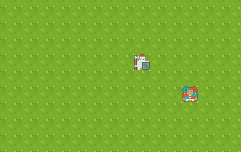
\includegraphics[width=0.5\textwidth]{data/06/33dede-9a84-458e-8ea0-5ae29bb9bc9c/screenshot-20200306-160024.png}
\end{center}\end{center}
\end{frame}
\section{Mit den Datentypen arbeiten}
\label{sec:org516dccc}
\begin{frame}[label={sec:org8332606}]{Strukturen als Datenpaket}
\begin{itemize}
\item Die Verwendung von Strukturen als \alert{eine Sammlung von
zusammengehörenden Variablen} ist an sich schon nützlich
\item Strukturen werden aber speziell dann ein mächtiges Werkzeug zur
Abstraktion, wenn die Verarbeitung von den darin enthalteten Daten
in Funktionen passiert.
\end{itemize}
\end{frame}
\begin{frame}[label={sec:org1faff1f},fragile]{Strukturen als Parameter von Funktionen}
 So wie sie einen {\color{solarizedYellow}\texttt{int} }als Parameter in eine Funktion schicken können,
können Sie auch eine Struktur als Parameter an eine Funktion
übergeben.
\begin{exampleblock}{Beispiel}
\begin{minted}[fontsize=\scriptsize,numberblanklines=false]{c}
#include <stdio.h>

typedef struct Complex {
  double real;
  double imag;
} Complex;

void print(Complex num) { printf("%f + %fi\n", num.real, num.imag); }

int main() {
  Complex c = {1.2, 0.234};
  print(c);
}
\end{minted}
\end{exampleblock}
\end{frame}
\begin{frame}[label={sec:org540bcb5},fragile]{Rückgabe von Strukturen von Funktionen}
 Genauso wie Sie einen {\color{solarizedYellow}\texttt{int} }von einer Funktion mittels {\color{solarizedYellow}\texttt{return}}
zurückgeben können, können Sie auch eine Struktur mit {\color{solarizedYellow}\texttt{return} }zurück
geben
\begin{exampleblock}{Beispiel}
\center
Nächstes Slide
\begin{center}\begin{center}
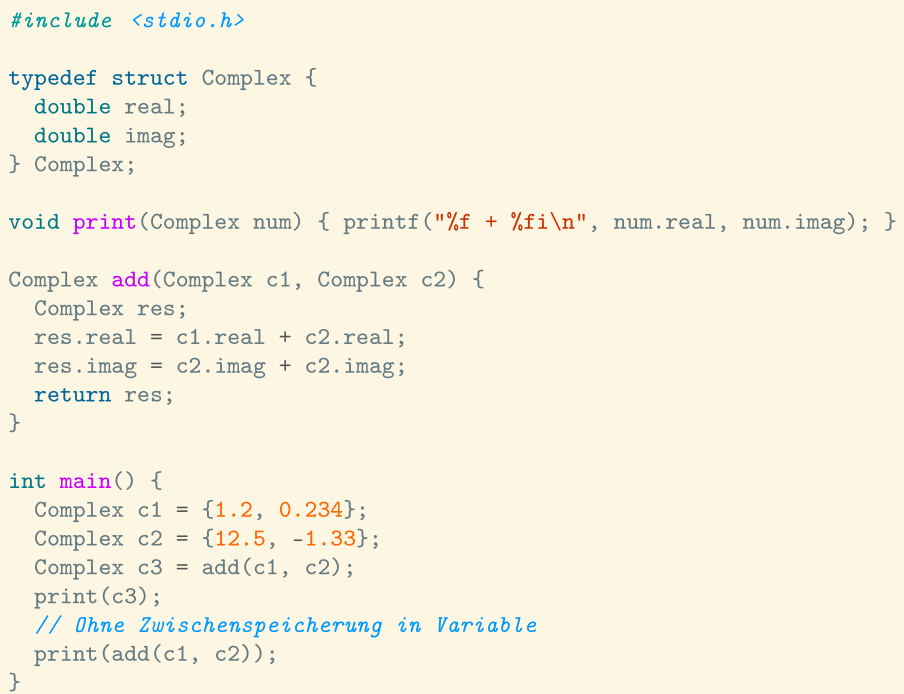
\includegraphics[width=0.3\textwidth]{data/b1/ec1282-fa9f-4a02-abc6-b8b219020ccc/screenshot-20200306-173506.png}
\end{center}\end{center}
\end{exampleblock}
\end{frame}

\begin{frame}[label={sec:orgeffb613},fragile]{Rückgabe von Strukturen von Funktionen --- Beispiel}
 \begin{minted}[fontsize=\scriptsize,numberblanklines=false]{c}
#include <stdio.h>

typedef struct Complex {
  double real;
  double imag;
} Complex;

void print(Complex num) { printf("%f + %fi\n", num.real, num.imag); }

Complex add(Complex c1, Complex c2) {
  Complex res;
  res.real = c1.real + c2.real;
  res.imag = c1.imag + c2.imag;
  return res;
}

int main() {
  Complex c1 = {1.2, 0.234};
  Complex c2 = {12.5, -1.33};
  Complex c3 = add(c1, c2);
  print(c3);
  // Ohne Zwischenspeicherung in Variable
  print(add(c1, c2));
}
\end{minted}
\end{frame}
\begin{frame}[label={sec:org962b235},fragile]{Rückgabe --- Beispiel ohne temporäre Variable}
 \begin{minted}[fontsize=\scriptsize,numberblanklines=false]{c}
#include <stdio.h>

typedef struct Complex {
  double real;
  double imag;
} Complex;

void print(Complex num) { printf("%f + %fi\n", num.real, num.imag); }

Complex add(Complex c1, Complex c2) {
  return (Complex){c1.real + c2.real, c1.imag + c2.imag};
}

int main() {
  Complex c1 = {1.2, 0.234};
  Complex c2 = {12.5, -1.33};
  Complex c3 = add(c1, c2);
  print(c3);
  // Ohne Zwischenspeicherung in Variable
  print(add(c1, c2));
}
\end{minted}
\end{frame}
\begin{frame}[label={sec:orgf519c29},fragile]{Rückgabe --- Beispiel komplett ohne Variablen}
 \begin{minted}[fontsize=\scriptsize,numberblanklines=false]{c}
#include <stdio.h>

typedef struct Complex {
  double real;
  double imag;
} Complex;

void print(Complex num) { printf("%f + %fi\n", num.real, num.imag); }

Complex add(Complex c1, Complex c2) {
  return (Complex){c1.real + c2.real, c1.imag + c2.imag};
}

int main() {
    print(add((Complex){1.2, 0.234}, (Complex){12.5, -1.33}));
}
\end{minted}
\end{frame}
\begin{frame}[label={sec:org989b13d},fragile]{Ändern der Werte einer Struktur innerhalb einer Funktion}
 Wenn Sie Strukturen als Parameter an eine Funktion übergeben, können
Sie die Werte darin zwar ändern, aber \alert{diese Änderungen haben keine
Auswirkungen außerhalb der Funktion}
\begin{exampleblock}{Beispiel}
\begin{minted}[fontsize=\scriptsize,numberblanklines=false]{c}
#include <stdio.h>

typedef struct Complex {
  double real;
  double imag;
} Complex;

void print(Complex num) { printf("%f + %fi\n", num.real, num.imag); }
void init(Complex num) { num.real = num.imag = 0.0; }

int main() {
  Complex c = {23.0, 42.27};
  init(c);
  // c ist immer noch 23.0 + 42.27i und nicht 0.0 + 0.0i !
  print(c);
}
\end{minted}

\begin{verbatim}
23.000000 + 42.270000i
\end{verbatim}
\end{exampleblock}
\end{frame}

\begin{frame}[label={sec:orgc7c7733},fragile]{Übergabe von Strukturen als Zeiger}
 Um Werte in einer Struktur nach aussen hin sichtbar zu ändern, muss
die Struktur als Zeiger an die Funktion übergeben werden
\begin{minted}[fontsize=\scriptsize,numberblanklines=false]{c}
#include <stdio.h>

typedef struct Complex {
  double real;
  double imag;
} Complex;

void print(Complex num) { printf("%f + %fi\n", num.real, num.imag); }
void init(Complex *num) { (*num).real = (*num).imag = 0.0; }

int main() {
  Complex c = {23.0, 42.27};
  init(&c);
  // c ist jetzt 0.0 + 0.0i !
  print(c);
}
\end{minted}

\begin{verbatim}
0.000000 + 0.000000i
\end{verbatim}
\end{frame}

\begin{frame}[label={sec:orgcc97762},fragile]{Zugriff auf Komponenten eines Strukturzeigers}
 \begin{itemize}
\item Der Zugriff mit einem Punkt nach dem Dereferenzieren (z.B.
{\color{solarizedYellow}\texttt{(*num).real}}) ist etwas umständlich.
\item Syntactic Sugar um das ganze leserlicher zu machen:
\begin{itemize}
\item Statt {\color{solarizedYellow}\texttt{(*num).real} }kann auch {\color{solarizedYellow}\texttt{num->real} }geschrieben werden
\end{itemize}
\end{itemize}
\begin{exampleblock}{Beispiel}
\begin{minted}[fontsize=\scriptsize,numberblanklines=false]{c}
#include <stdio.h>

typedef struct Complex {
  double real;
  double imag;
} Complex;

void print(Complex num) { printf("%f + %fi\n", num.real, num.imag); }
void init(Complex *num) { num->real = num->imag = 0.0; }

int main() {
  Complex c = {23.0, 42.27};
  init(&c);
  print(c);
}
\end{minted}
\end{exampleblock}
\end{frame}
\begin{frame}[label={sec:org6dc2091},fragile]{Übung}
 Schreiben Sie folgende Funktionen für unser auf Strukturen umgeschriebenes Spielebeispiel:
\begin{description}
\item[{{\color{solarizedYellow}\texttt{draw\_figure}}}] Zeichnet die Figur mit der richtigen Grafik an der richtigen Stelle
\item[{{\color{solarizedYellow}\texttt{are\_colliding}}}] Übernimmt zwei Figur-Strukturen und überprüft ob diese gerade kollidieren
\item[{{\color{solarizedYellow}\texttt{move\_up}}, {\color{solarizedYellow}\texttt{move\_down}}, {\color{solarizedYellow}\texttt{move\_left}}, {\color{solarizedYellow}\texttt{move\_right}}}] Bewegt eine
Figur nach Oben, Unten, Links, Rechts und stellt sicher, dass
sich diese nicht vom Spielfeld bewegt
\end{description}
\begin{center}\begin{center}
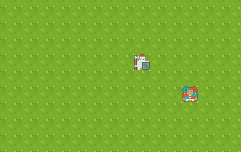
\includegraphics[width=0.3\textwidth]{data/06/33dede-9a84-458e-8ea0-5ae29bb9bc9c/screenshot-20200306-160024.png}
\end{center}\end{center}
Verwenden Sie die geschriebenen Funktionen an geeigneter Stelle in
unserem Spiel
\end{frame}
\end{document}